\documentclass[a4paper]{jpconf}
\usepackage{graphicx}
\bibliographystyle{iopart-num}
\usepackage{citesort}

\begin{document}
\title{The True Cost of Data Access in ATLAS}

\author{VUKOTIC, Ilija$^1$, GARDNER JR, Robert William$^1$, MCKEE, Shawn$^2$ }

\address{$^1$ University of Chicago, 5620 S Ellis Ave, Chicago IL 60637, USA}
\address{$^2$ University of Michigan, ATLAS Group}

\ead{ivukotic@cern.ch}

\begin{abstract}
  As new ways of accessing and transferring data distributed over the grid emerge (XRootD-based storage networks, dynamic http federations, etc.) and as the quantity of data grows, a number of challenges are presented to both the application layer and the supporting compute, network and storage infrastructures. Clearly network links between compute and storage systems remain the leading determinant for determining accessibility and performance between client and server. Indeed a number of systems to probe the network and aggregate information about transfers have been deployed to characterize bandwidth, latency and overall throughput between sets of endpoints. We describe combining these and other information sources into a time-dependent cost-of-data-access matrix. This matrix, in combination with other performance indicators, can be used to directly support job brokering and data distribution decisions. More importantly, it can be used as an input to dynamically evolve ATLAS data paths using advanced network protocols such as OpenFlow where they are implemented. We review models of the transfer prioritization, quality-of-service differentiation, and other technologies and their effects on resource utilization.
\end{abstract}

\section{Introduction}

In 2011 ATLAS~\cite{atlas} recoded RAW data at up to 450 MB/s and by the end of the running period has collected 5.61 fb$^{-1}$ of data ($1.58\times10^{9}$ events - 3.38~PB) at 7 TeV center of mass energy proton-proton collisions. In addition 1.25 times as much of the derived data formats has been produced~\cite{boris}. In the same period 3.5 billion events (9.78~PB) of Monte Carlo data has been produced. All of this requires an enormous computing resources. While it is relatively easy to account for the resources consumed at the run and stream level, to act upon the system a much more detailed information is needed. Knowing how changes in average interaction rate affect CPU and memory consumption of each algorithm, or how it influences size of each stored collection, gives a predictive power needed to plan the future data taking parameters and provision in time for the computing resources.

The main goal of this system is to provide the following information:
\begin{itemize}
	\item size of all the objects that ATLAS stores in all officially produced data files.
	\item timing of all the algorithms, tools and services used during official data production, simulation, and reconstruction.
	\item CPU time, wall clock time, memory leakage and other per job information 
\end{itemize}

% \begin{figure}[ht]
% \begin{minipage}[b]{0.5\linewidth}
% \centering
% 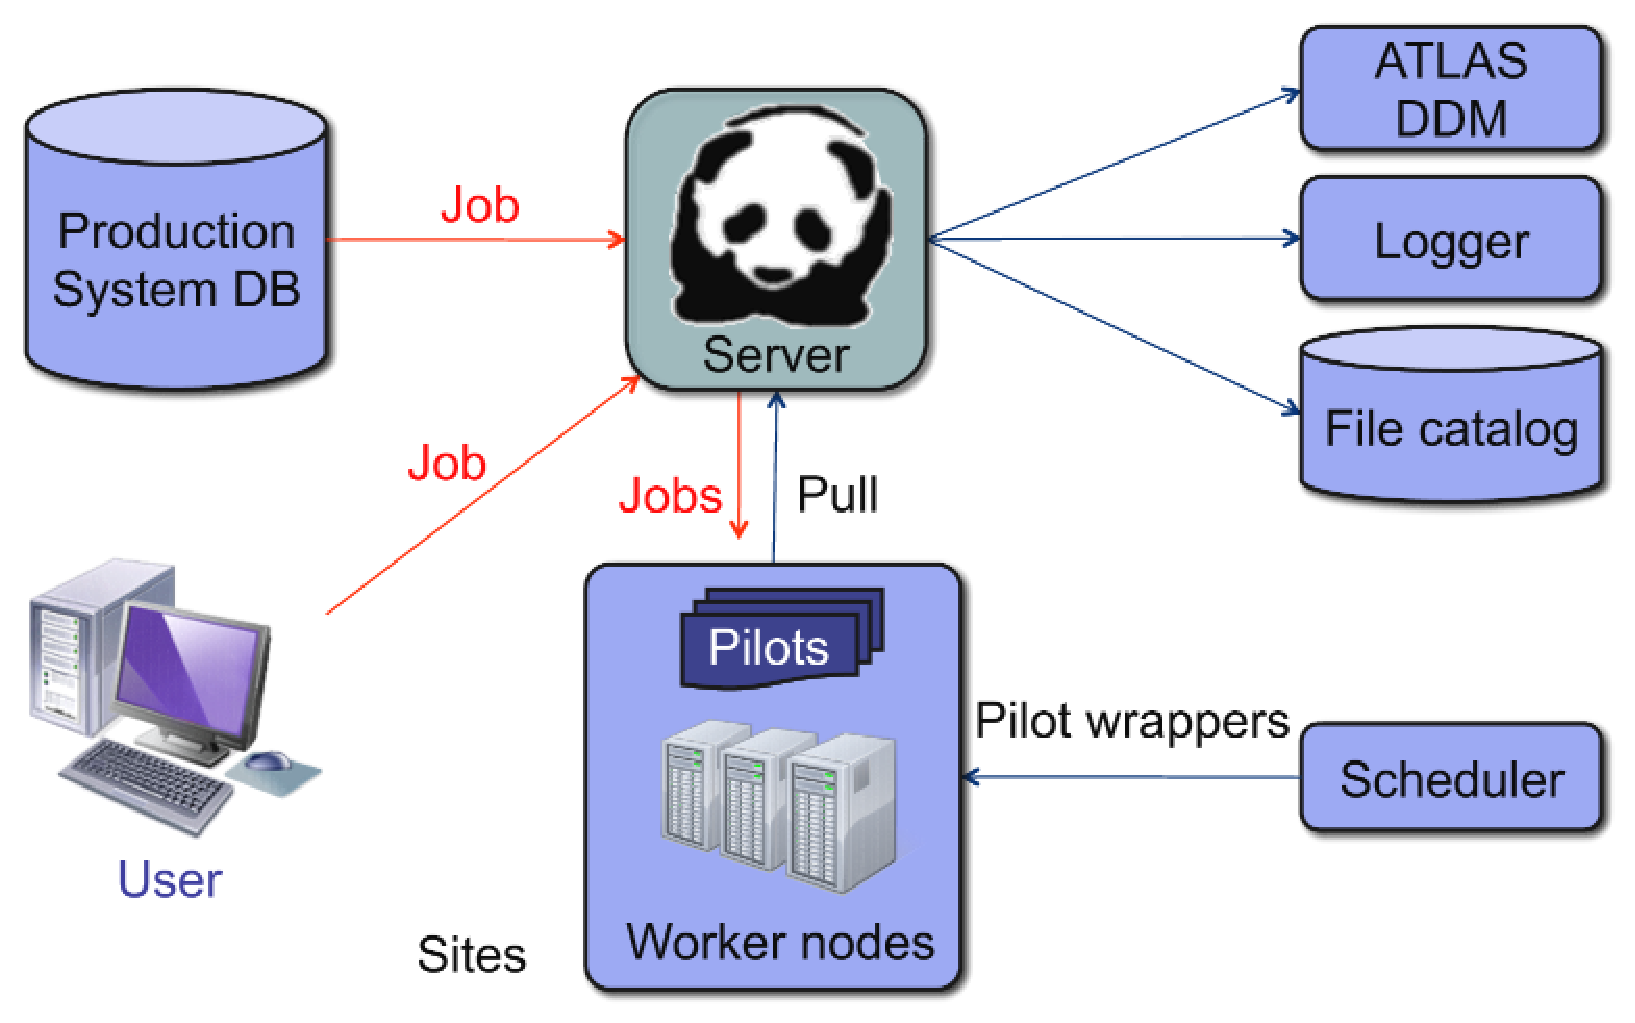
\includegraphics[width=\columnwidth]{panda.eps}
% \caption{The ATLAS Production and Distributed Analysis system (PanDA) is workload management system, managing ATLAS distributed production requirements.}
% \label{fig:panda}
% \end{minipage}
% \hspace{0.5cm}
% \begin{minipage}[b]{0.5\linewidth}
% \centering
% 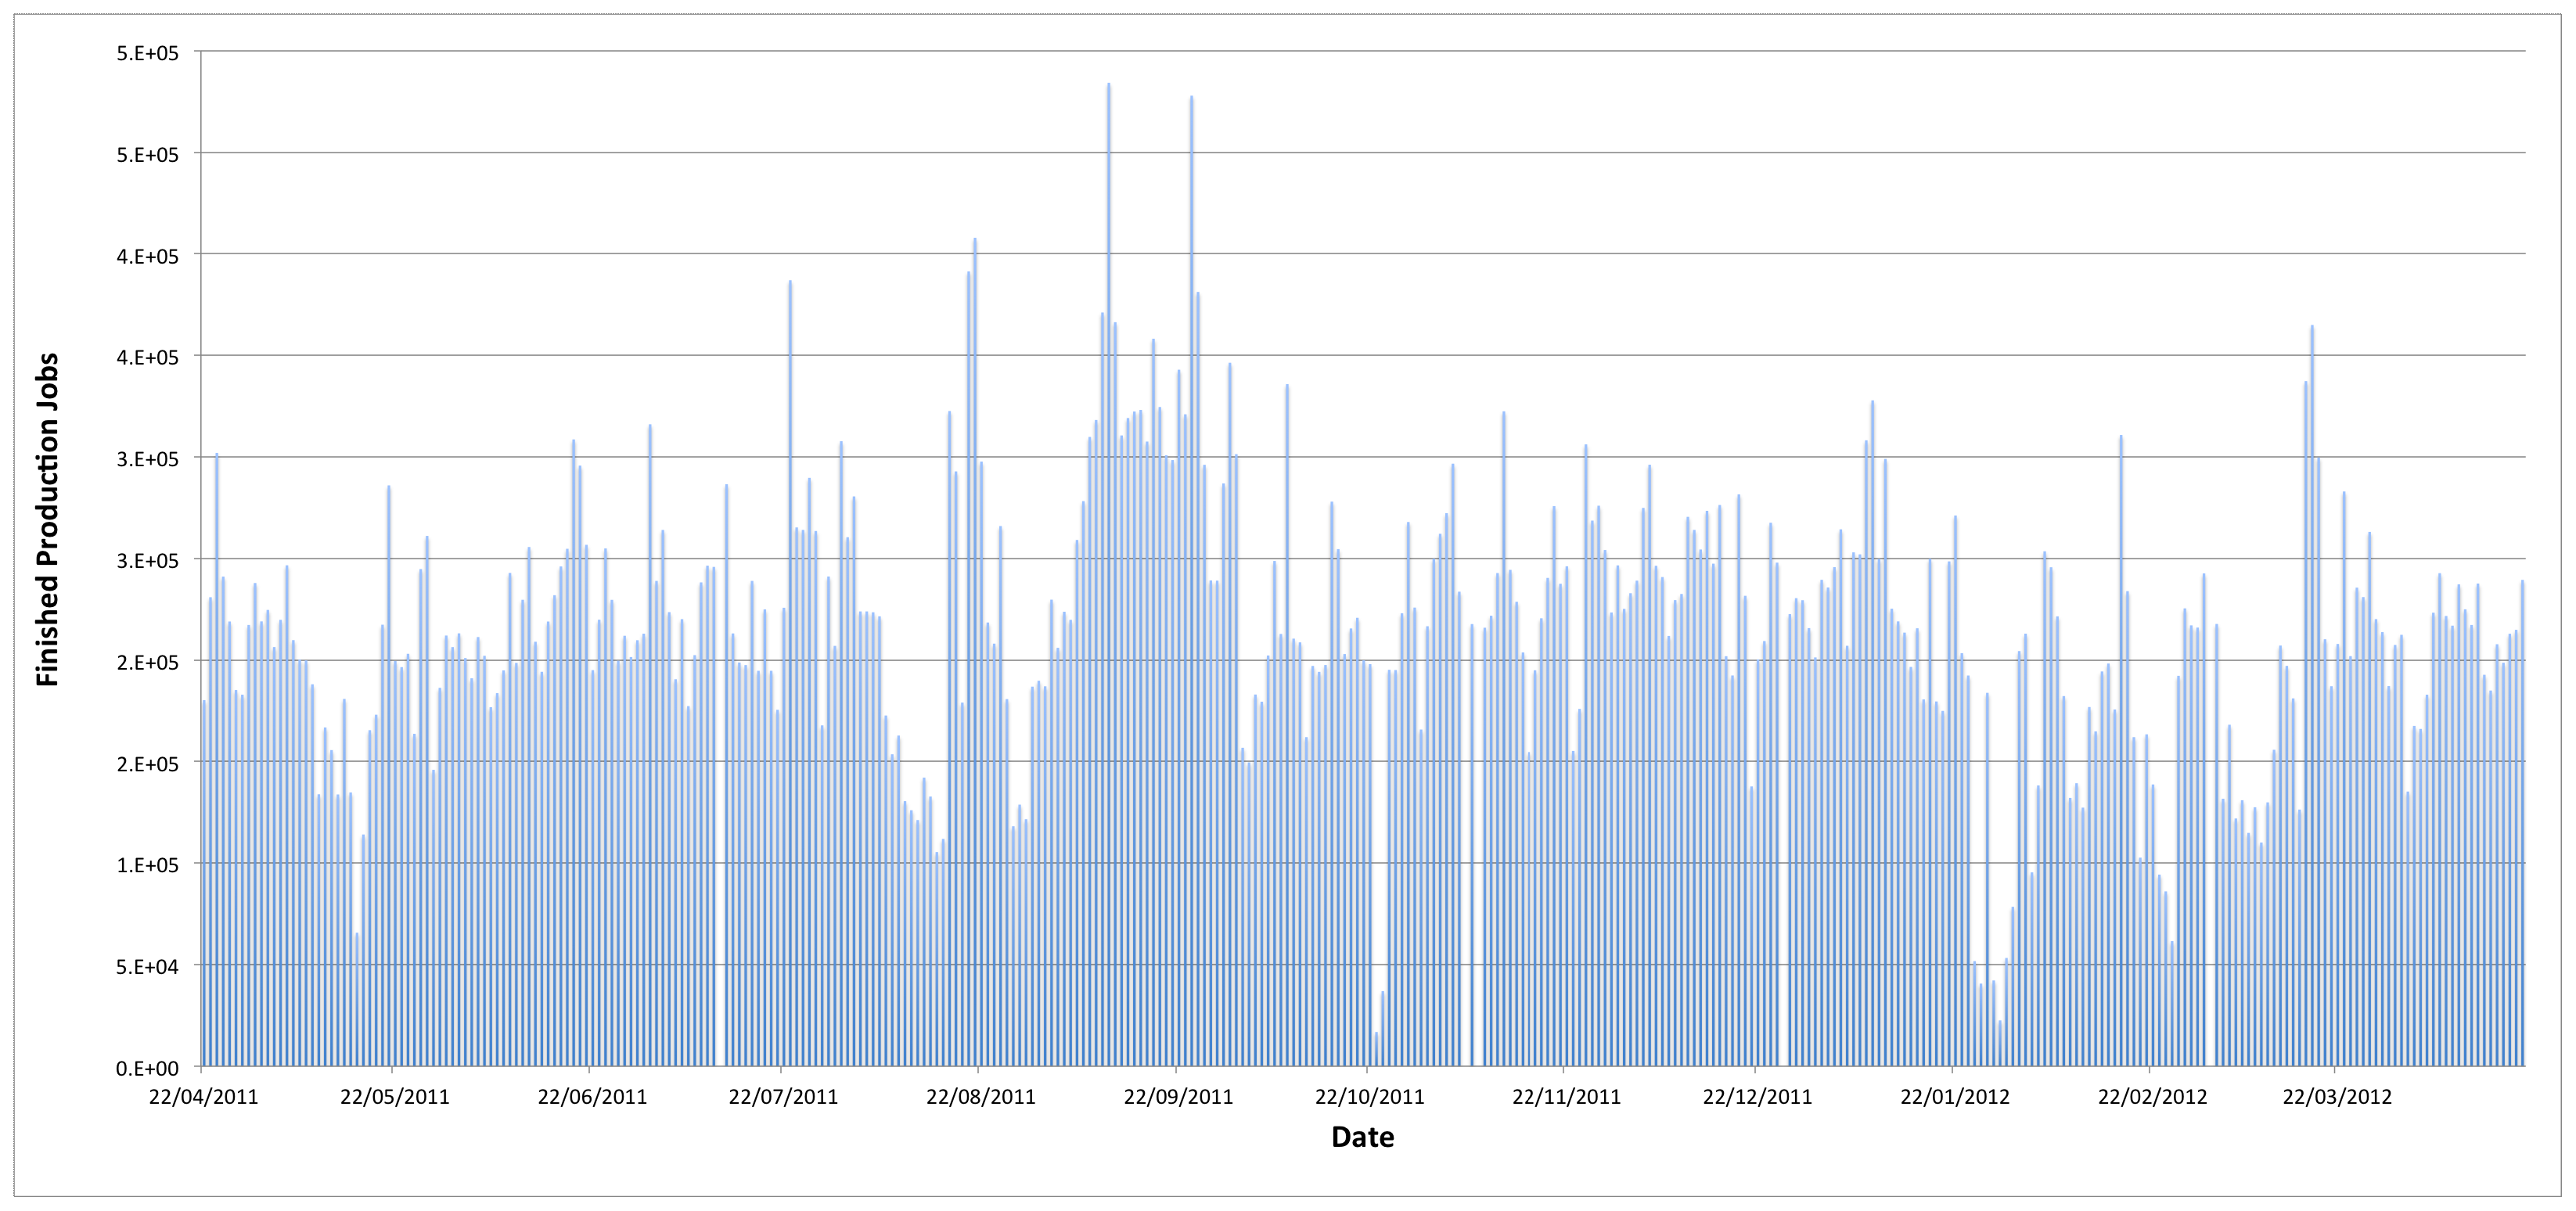
\includegraphics[width=\columnwidth]{jobsLastYear.eps}
% \caption{Number of running ATLAS production jobs per day during last year.}
% \label{fig:jobsLastYear}
% \smallskip 
% \end{minipage}
% \end{figure}

% \begin{figure}
%   \centering
%   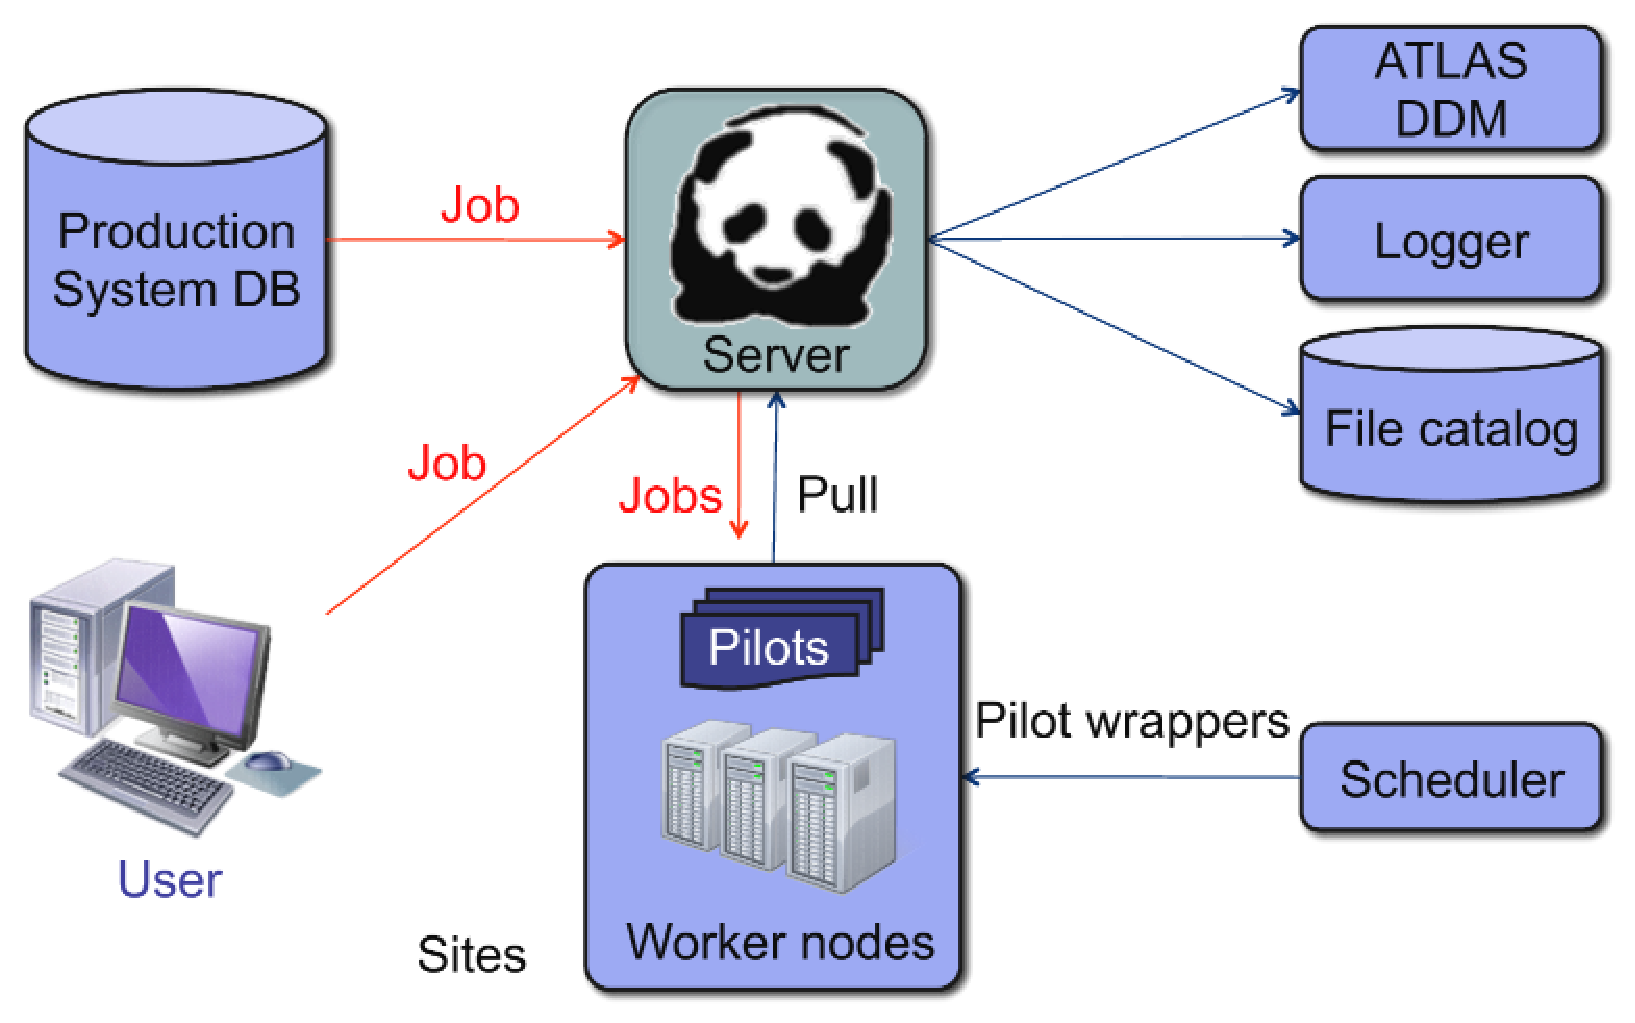
\includegraphics[width=0.5\columnwidth]{panda.eps}
%   \caption{The ATLAS Production and Distributed Analysis system (PanDA) is workload management system, managing ATLAS distributed production requirements}
%   \label{fig:panda}
% \end{figure}

This information will be used:
\begin{itemize}
	\item by performance experts to identify places where optimization will be most beneficial
	\item by management to determine current resource needs and to extrapolate for future running parameters
	\item by reconstruction shifters to continuously monitor changes in resource consumption
	\item example 1: find all the persistent objects not written out in last 1 year and remove them from the code.
	\item example 2: find all the unneeded persistent objects written out.
	\item example 3: find all the algorithms, tools or services not needed in a particular transformation step.
	\item example 4: estimate resources needed for a particular MC or real data production - reconstruction. 
\end{itemize}


\section{Framework}


In this document we will use term {\bf task} to signify an operation (eg. reconstruction) on the data set containing one or more files and {\bf job} to signify part of the task usually executed on one core and one input file. While jobs are usually very complex and involve multiple execution steps they are atomic operations ie. we consider job as failed in case of error in any part of it and all of its results are discarded.

The production system is schematically presented in Figure~\ref{fig:sysschema}. It is composed of two main parts: the Tier-0~\cite{tier0} and the grid Production System.

\begin{figure}
  \centering
  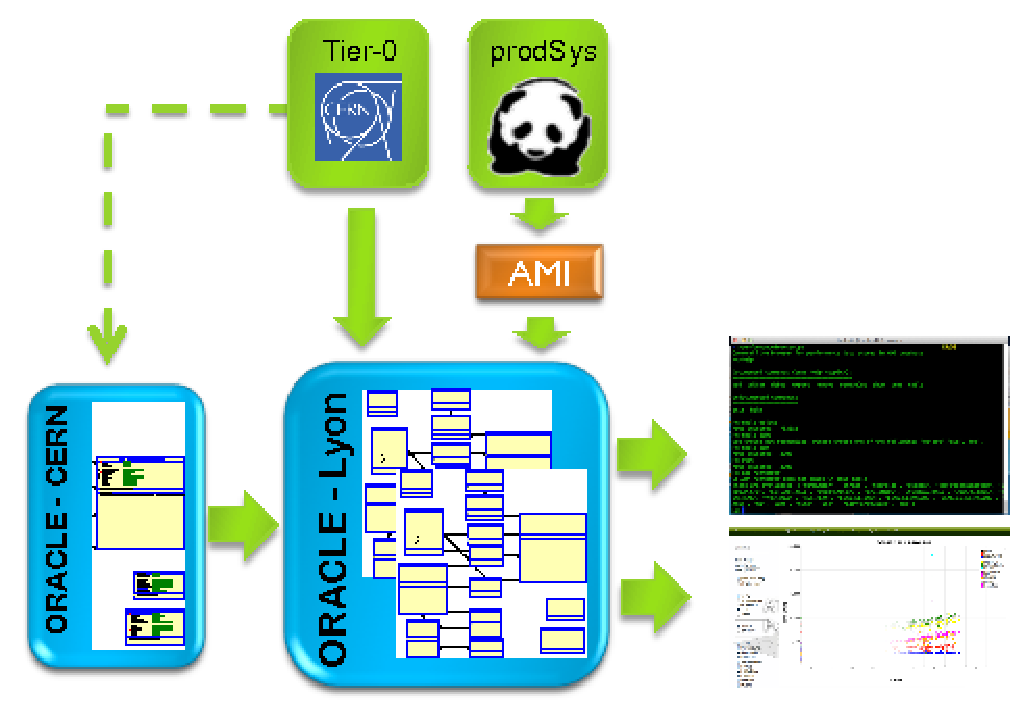
\includegraphics[scale=0.6]{sysschema.eps}
  \caption{Organization of the Atlas resources usage monitoring system.}
  \label{fig:sysschema}
\end{figure}

The Tier-0 having around 6000 processing cores is tasked with the initial real data reconstruction. It also reconstructs all the special streams: calibration, debug, express etc. As a calibration loop has to be finished inside 36 hours long delays are not allowed. Since jobs take roughly 10 hours even one failed job can introduce serious delays. For this reason failing a job due to resource monitoring is not an option, any problem in monitoring is just reported and the transform continues.

The grid based production system PanDA~\cite{panda} can be used for both reconstruction of real data and all the steps of MC production.
It is currently used at over 130 sites world-wide and currently running in average 200 thousand production jobs per day as can be seen in Figure~\ref{fig:jobsLastYear}. The system is also capable of handling user analysis jobs. While requirements on delays are not as strict as at Tier-0, job failing due to monitoring is again not acceptable since even very small percentage of failed jobs would mean a significant overhead for the production shifters.  


\begin{figure}
  \centering
  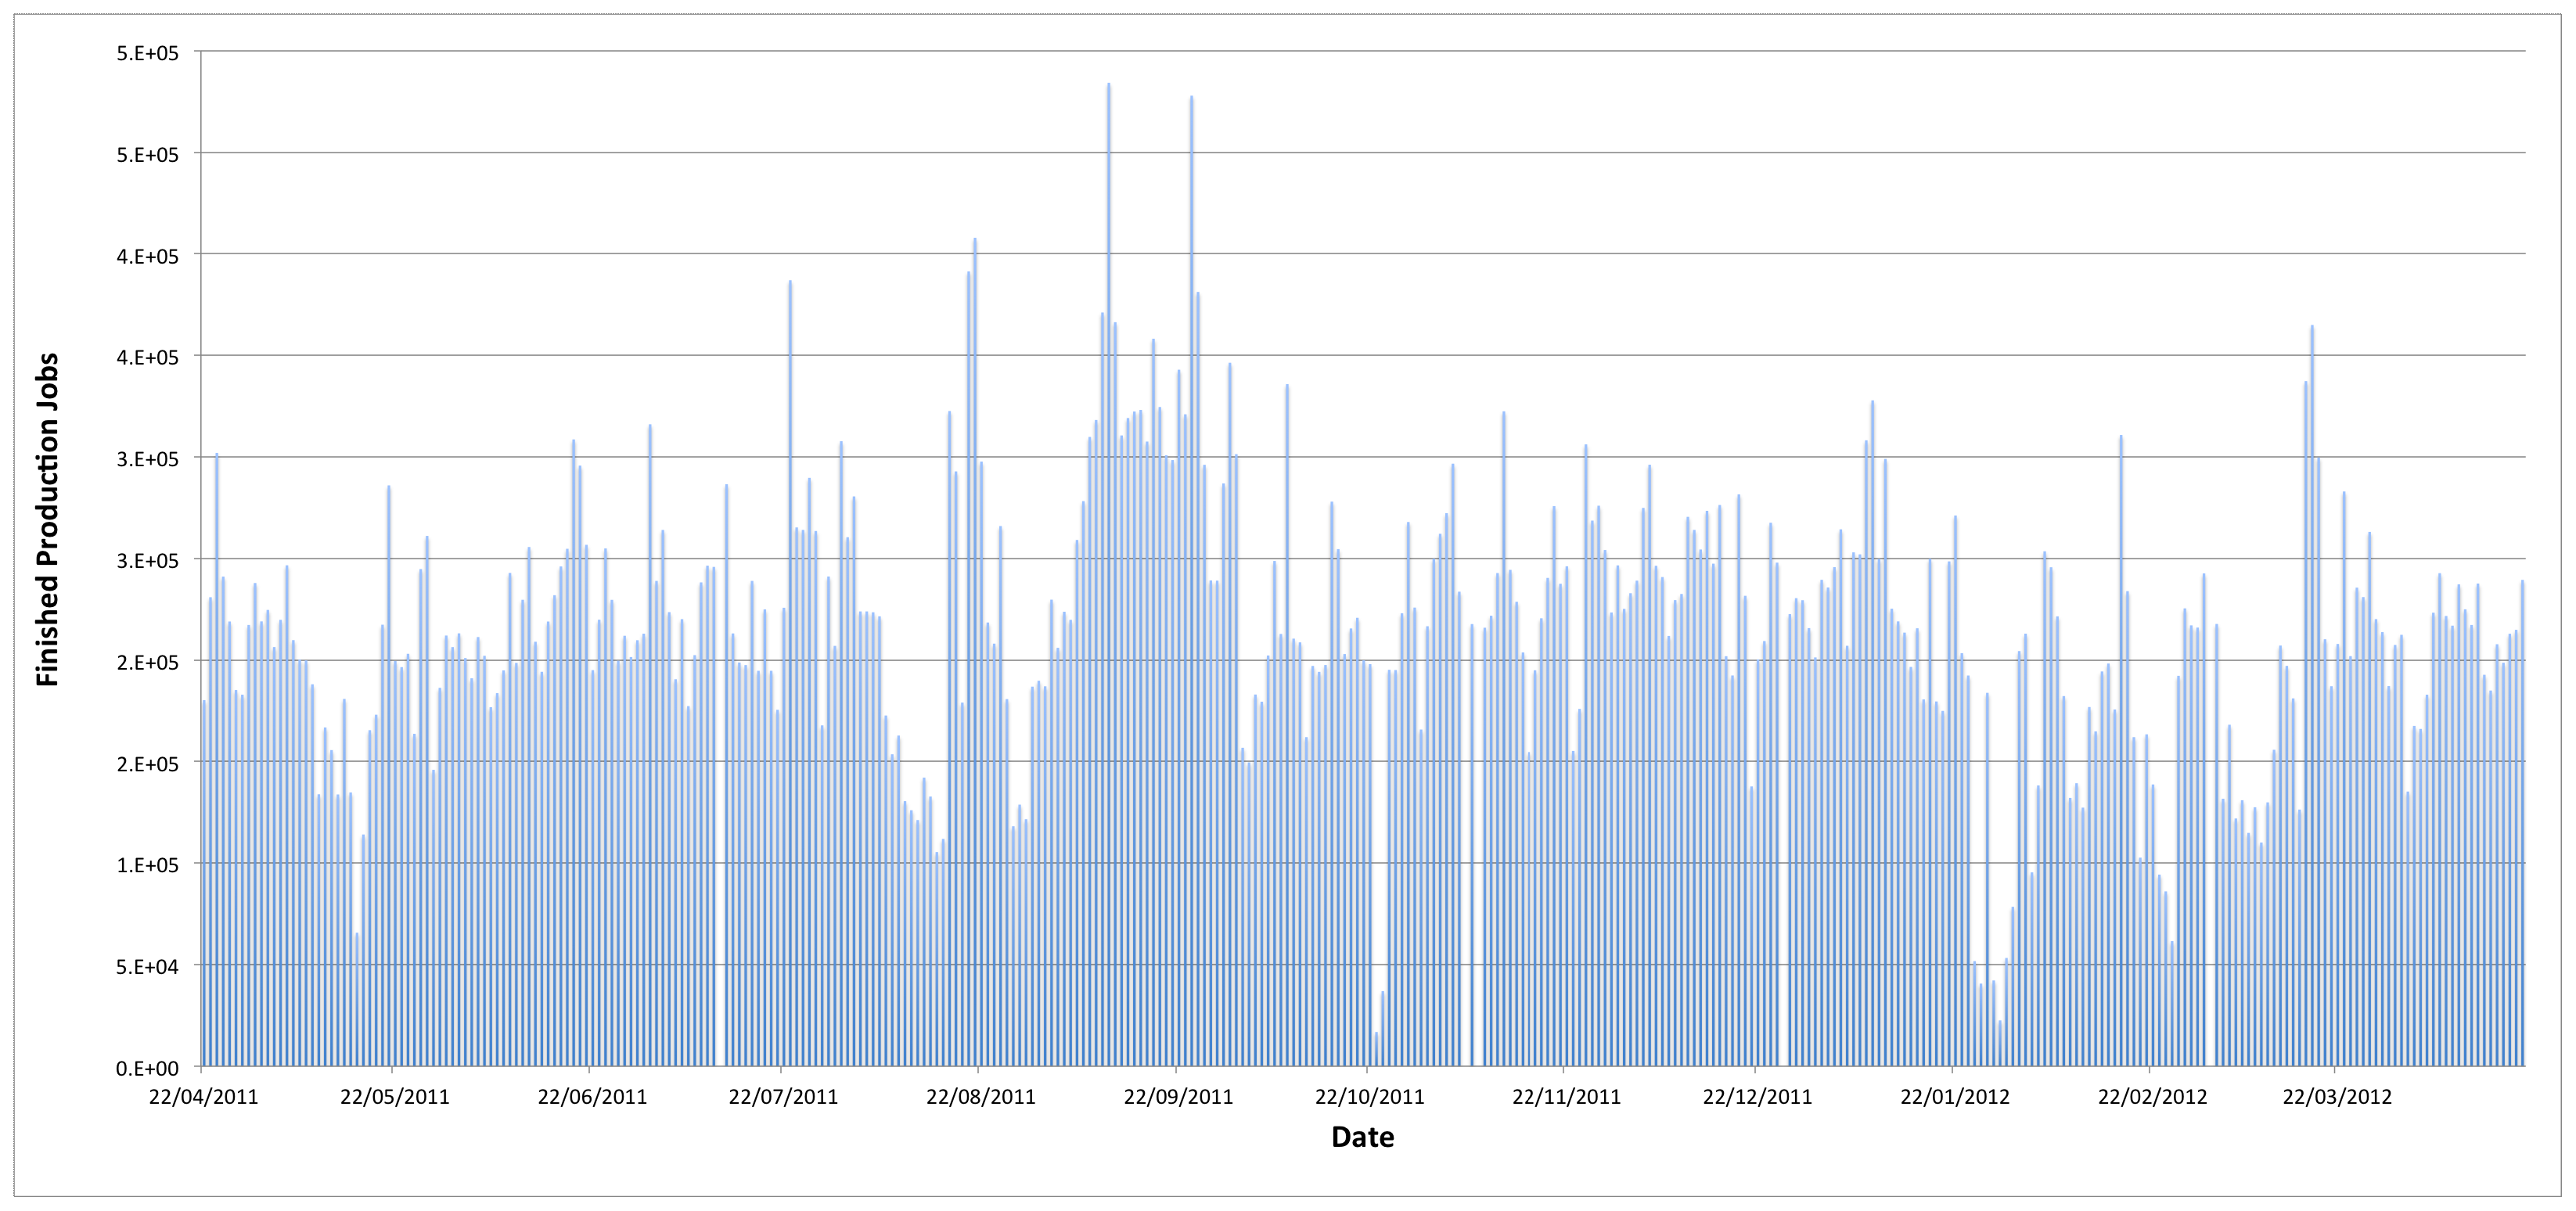
\includegraphics[width=\columnwidth]{jobsLastYear.eps}
  \caption{Number of running ATLAS production jobs per day during last year.}
  \label{fig:jobsLastYear}
\end{figure}


Allowing monitoring to quietly fail can lead to not having resource usage information from all of the events. It can also happen that a job fails after it already sent part of the information to the DB. As the job is restarted, that leads to these events having twice the statistical weight. Both of these effects should not matter for most of applications. In case of MC collecting information from even small percentage of jobs is sufficient. We assume that sampling just 20\% of all the jobs will give us good enough cross-section of hardware and middleware resources used.  For the real data majority of jobs is good enough. While the Tier-0 resources are uniformed, time dependent changes in for example trigger settings, average number of interactions per bunch crossing, etc. can lead to big fluctuations in amount of resources used.
    
All of the monitoring system is composed of 4 functional parts: information collection, data transport, data storage, and visualization. We will briefly describe each.

\subsection{Data collection}
The first problem we had to solve is how to distinguish production tasks/jobs to monitor. An additional option (\verb#--uploadToAmi=<probability>#) triggers collection and upload of the information with a given probability. This option is usually coming from the AMI~\cite{ami} database via so called ami tag. At Tier-0, production jobs are identified by a special environment variable, while at prodSys jobs are monitored if users grid certificate has a production role in ATLAS VO.   

All of the production jobs are actually executions of the same script (\verb#Reco_trf.py#) with different parameters. The parameters define input and output files, calibration constants etc. The reco transform executes an appropriate sequence of Athena~\cite{athena} sub-jobs. As we need information collected from each of these sub-jobs, the transform itself is the place to collect the data.

While this can be changed for now we settled at:
\begin{itemize}
	\item stored object size is obtained from PoolFile.py. This is a ROOT~\cite{root} based tool that opens output root files and returns names, sizes and number of entries of all the collections stored (collection is the smallest object that can be read from ATLAS AOD or ESD file).
    \item algorithm timings are currently obtained from PerfMonSD tool. (Data collected before 1st April were obtained through ChronoSvc, part of the Gaudi framework~\cite{gaudi}).
    \item per job information (vmem, rss etc.) is obtained from operating system, not directly but again through the PerfMonSD.
\end{itemize}

An additional information which is not known at the job level but is needed, is collected by and uploaded into the data base by a cron job running every hour. These are: $<{\mu}>$  - average number of interactions in a bunch crossing during the run, run luminosity, duration, number of events, "use" flag - manually set data quality flag, and ReadyForPhysics - flag obtained from AMI db. 
	
		
\subsection{Data transport}

    Normally Tier-0 collected data are sent directly to Oracle DB in Lyon. The same Oracle servers are used by the AMI. In case the Lyon Oracle DB is unreachable the data are sent to a special Oracle DB situated in CERN. This DB schema is quite different and has only the tables and stored procedure needed to temporarily store the data. When normal DB conditions are re-established in Lyon, the data from CERN are retrieved automatically. 
	prodSys (grid) jobs data are also stored in the AMI DB in Lyon, this time not directly but through the AMI framework. As high throughput is needed the special AMI commands are provided. Special commands required: 
\begin{itemize}
	\item Extensive profiling.
	\item Adding a class to the low level Oracle JDBC level in AMI to handle stored procedures.
	\item Wrapping it in an "AMICommand" with minimum argument coherence checks (as we expect that calls will be generated by a robot, not a person).
	\item One command per stored procedure.
	\item change of the standard AMI Command behavior which is to return all the input arguments to the user along with the result, thus cutting the network time. 
	\item Authentication is done via VOMS.
\end{itemize} 
Not to unnecessarily stress AMI, checks that VOMS proxy has production role are done already on the client side. 

Currently there is no backup solution in case of problems with AMI. In both cases it is guaranteed that if upload of collected information fails for whatever reason it will fail quietly and jobs will finish normally. There is a window of 60 seconds in which all of the data collection and delivery has to be done.

\subsection{Data storage}

Rate of information collection, amounting to around 40 GB per day, presents the biggest challenge of this project. In order to fit into shared and very limited Oracle server resources required a special design and detailed optimization of the database schemes. It is important to notice that we are interested in resource utilization per task, task being defined by the input dataset, transform executed and set of processing variables (ami tag). As we are not interested in a detailed information from each individual jobs in that task, information sent to the DB by the jobs has to be summarized. This results in reduction of information stored by factor equal to number of jobs in the task (usually more than thousand).  
\begin{figure}
  \centering
  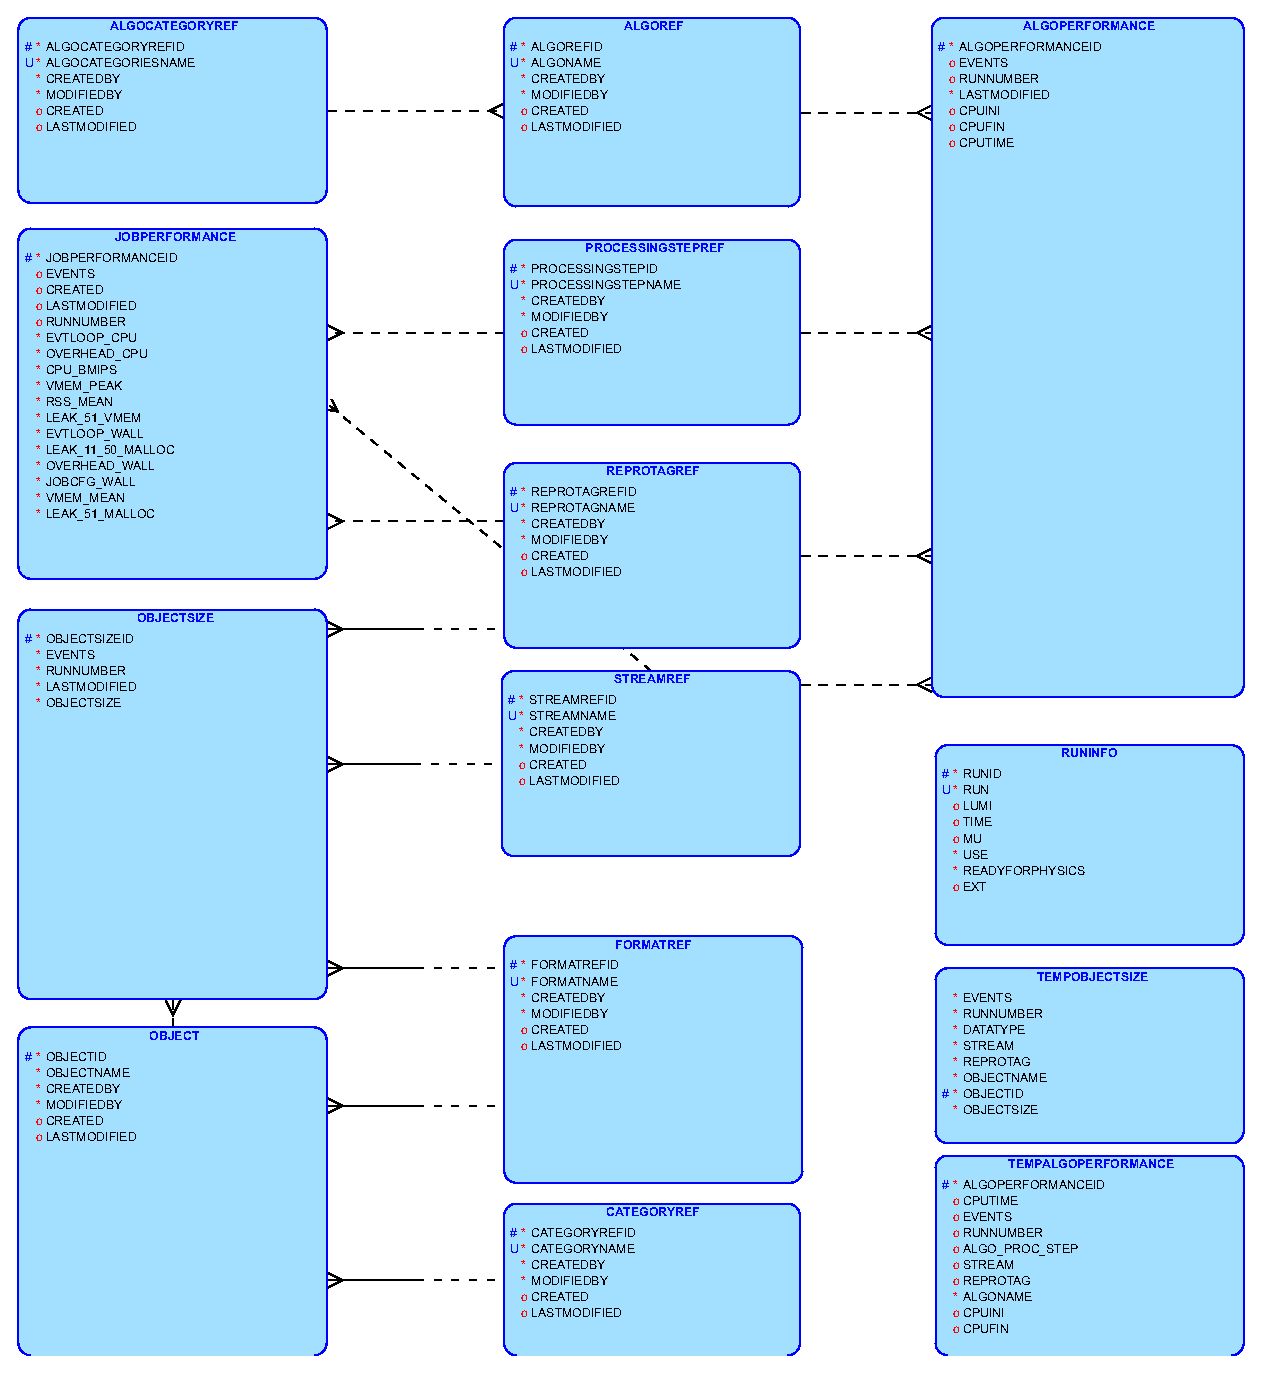
\includegraphics[width=\columnwidth]{performanceInAMIdesign.eps}
  \caption{Data base schema used to store the resource data. Fail-over schema consists just of "buffer" tables and the same stored procedures that accept the data.}
  \label{fig:dbschema}
\end{figure}
Oracle database schemes for both Tier-0 and prodSys data are identical. Their logical model can be seen in Figure~\ref{fig:dbschema}. The most important database design decision was to have "buffer" tables for both object size and algorithm timing data. These tables have no indices and no constrains of any kind. This makes bulk inserts into them extremely fast, and also evens the load on the DB servers. Once a week tables are resized for performance reasons. Information collected is added to appropriate rows of the "real" tables using stored procedures executed every 2 minutes. Both stored procedures are optimized by changing row based with table based sql commands wherever possible. The two largest "real" tables are also optimized by partitioning them according to run number.
 

	
\subsection{Data mining}

Multidimensionality and size of the data collected warranted providing multiple ways to do data analysis and data mining. The most basic functionality is provided by the AMI itself. There are two ways to use AMI for this purpose. Via simple web interface any registered AMI user can browse the tables and users with special privileges have update and delete rights, too. This is useful for simple lookups or changes for example: assigning a collection to different category. Second way is to construct custom queries that can be executed both from AMI web interface and from command line using pyAMI commands. Both ways are limited to returning less than 16000 rows.

One important aspect of analyzing data is a categorization of both the collections written in ATLAS data files and also all of algorithms, tools and services. Two python scripts, sorting based only on object names, are provided for this purpose and supported by an Event Data Management expert.  

A specially developed command line interface, written in python and based on pyAMI, provides full access to data, possibility to select parts of data, apply cuts and finally export a manageably sized portion of data to either CSV or ROOT files.
   
Finally a web interface (done in asp, jquery and highchars), shown in Figure~\ref{fig:webcapture} provides a simple and fast way to visualize the most important data. The page is designed not only with experts in mind, but also for shifters that would ideally monitor several of most important plots for unexpected changes.  

\begin{figure}
  \centering
  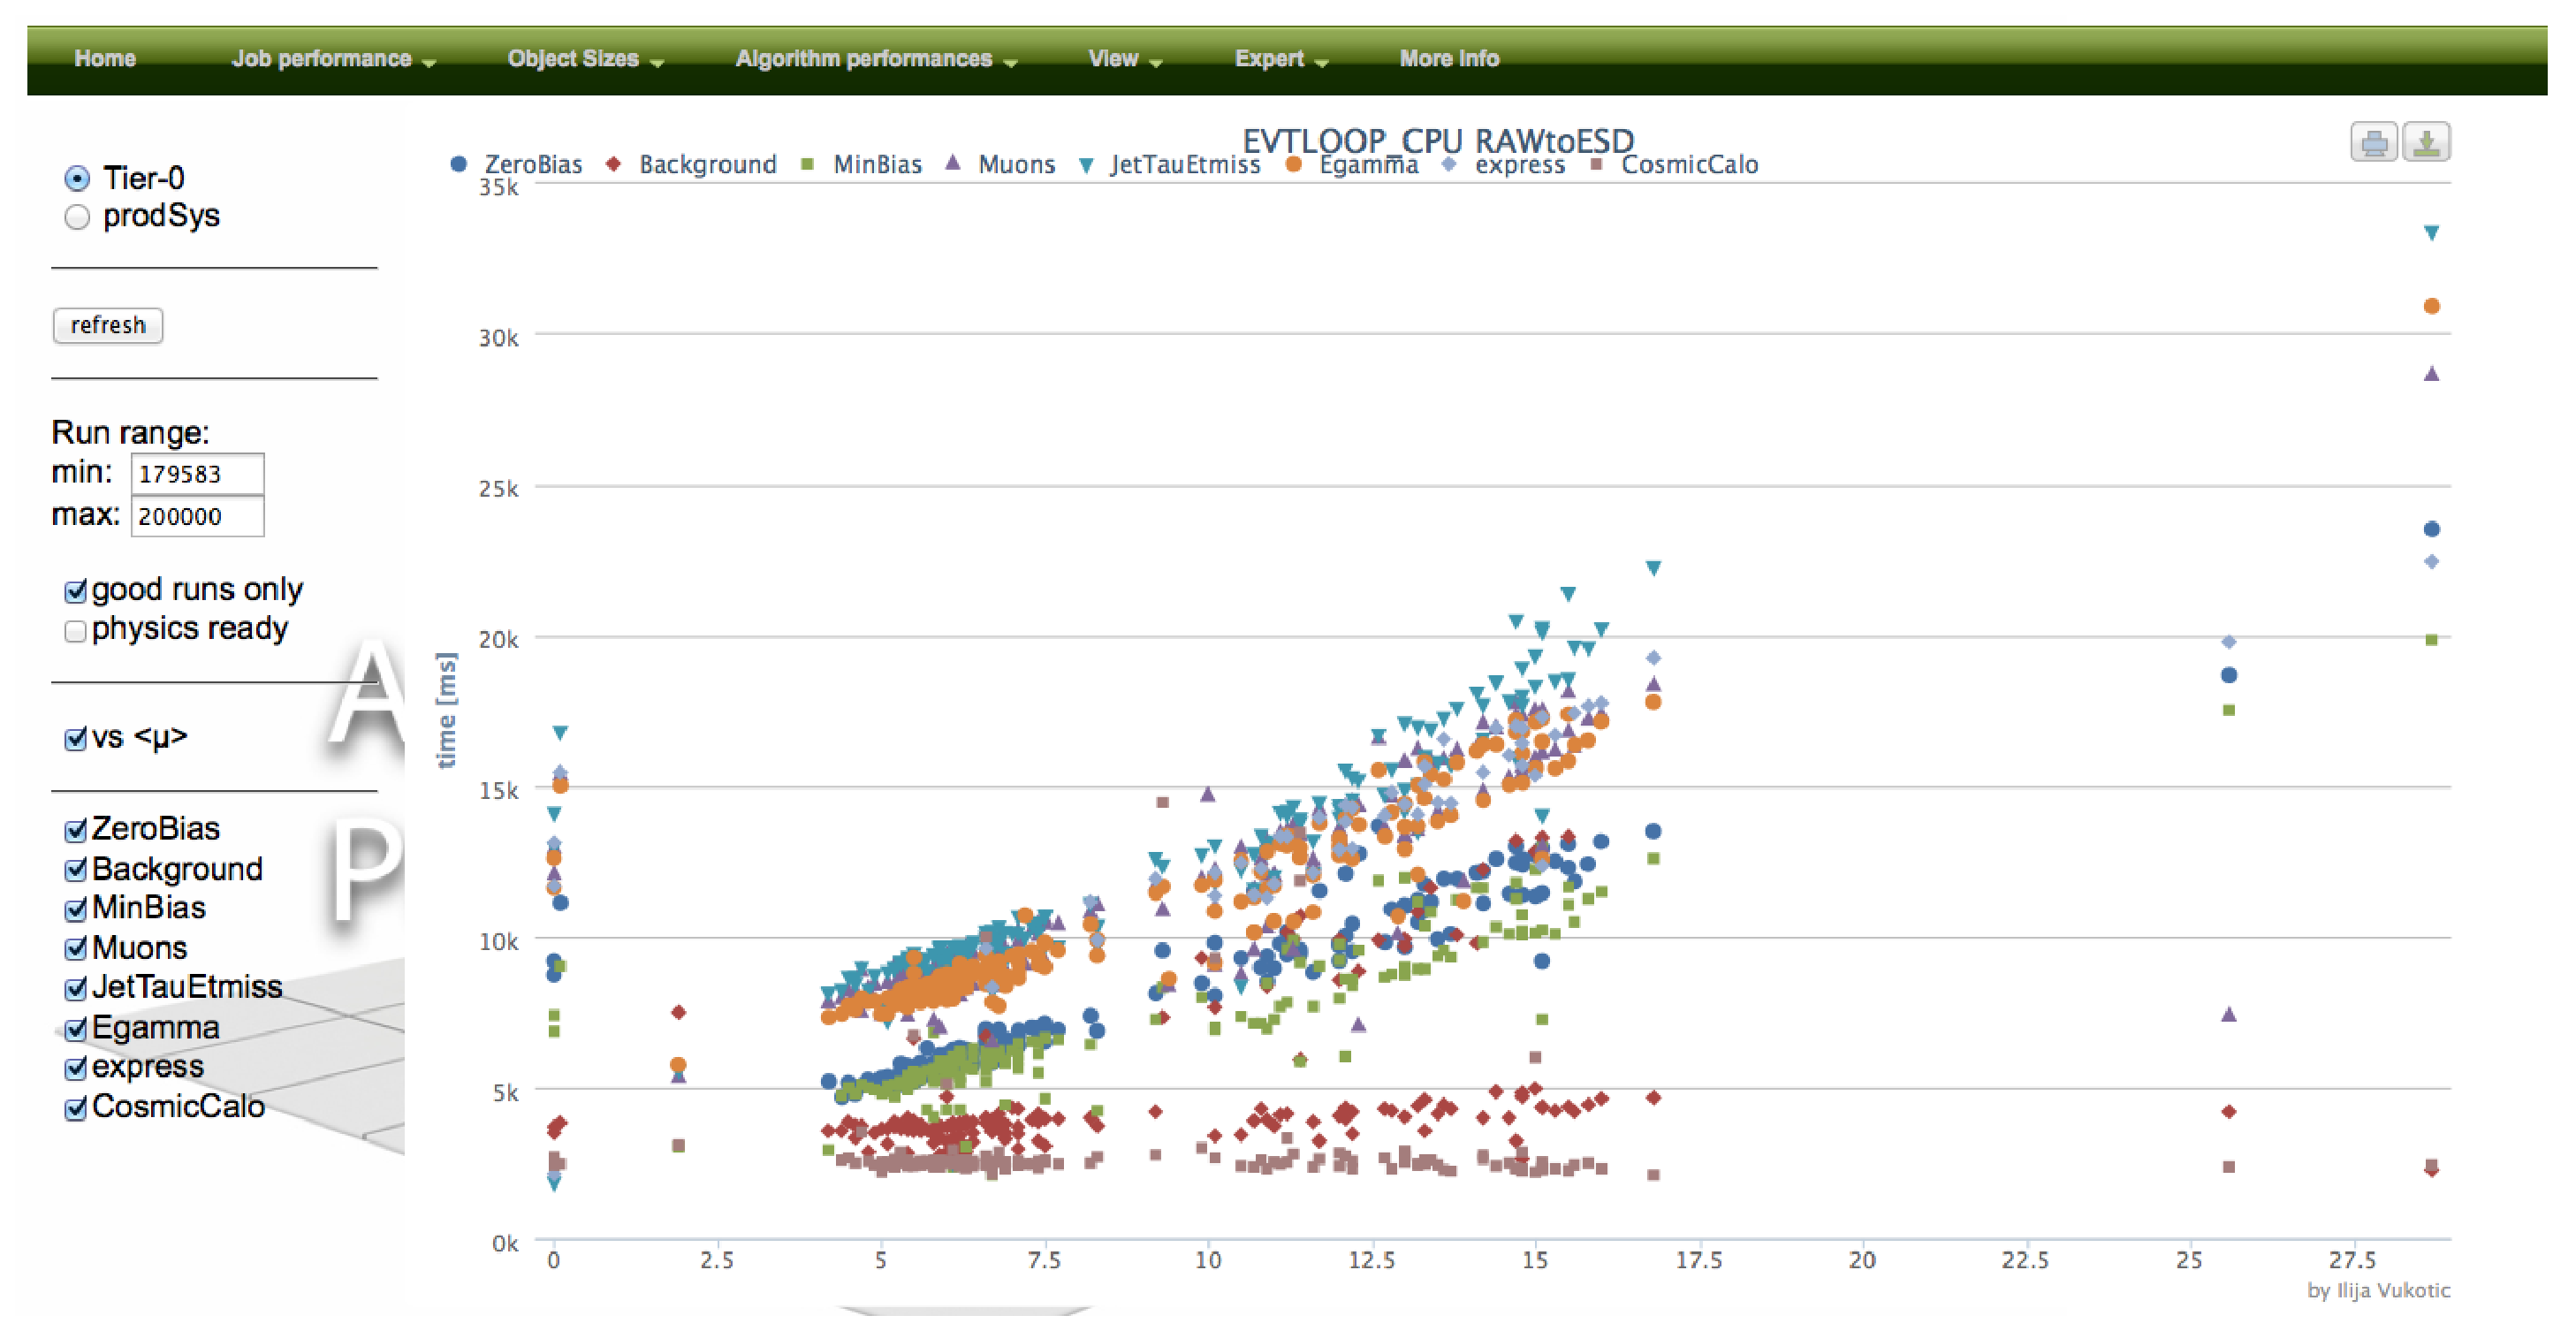
\includegraphics[width=\columnwidth]{webcapture.eps}
  \caption{Web interface allows for a fast and convenient access to all of the information collected. For a custom data analysis a command line interface allows for browsing the DB, cut application, and data export to CSV and ROOT files.}
  \label{fig:webcapture}
\end{figure}


\section{Performance in 2011}
Even with a very short development time and limited possibilities to debug the system, running it proved rather smooth. There was a period when the data where not collected due to un-orderly crash of all the Oracle servers in Lyon and a few tasks got unexplainably stuck. Additionally, soon after start of the 2011 data taking period it was discovered that cx\_oracle connections which are used in a forked thread do not close properly - even server process related to it is stopped, it still keeps connection opened. This in turn can breach the limit on number of open connections set on server. The problem was solved by always opening, using and closing oracle connections in the same thread.
From all the runs that were monitored in the year 2011, the system collected information on 97.3\%. XXX
Standalone measurements showed that time to upload all the information ranges from 150-300~ms, negligible in comparison to duration of jobs. To test potential of the system to accept the data from the production system, a hyper-threaded program was used to stress the system by uploading dummy data with twice the expected upload rate (equivalent of 500 000 concurrent production jobs). Even that was still giving less than 10\% load on the DB instance dedicated to the system.


\section{Conclusion}
Experiments requiring enormous computing resources are always in need of system to monitor resource usage and provide fast, full, and detailed analytics. The system described proves that even at the scale of ATLAS experiment with hundreds of thousands of concurrent, world-wide distributed jobs, a relatively simple but highly optimized system with an Oracle DB back-end, can do the job without resorting to much more complicated solutions (both to set up and to support).

\section*{References}
\bibliography{ivukotic_CHEP2013}
  

\end{document}



